Entriamo ora più nel dettaglio per quella che la teoria etichetta \textit{coppia coniugata acido-base}. Va da precisare infatti che, similmente a quanto dicevamo per le redox, dove non può esistere un ossidante se non c'è contestualmente il riducente (ossia se una specie perde elettroni è indispensabile che questi vengano acquistati da un'altra specie), per gli acidi e le basi è necessario che, affinché una specie assuma il comportamento di acido, si trovi in presenza di una base.

Secondo Br\"{o}nsted-Lowry, se c'è una specie che cede un protone ci vuole una specie che acquisti questo protone. Quindi non c'è un acido o una base, ma abbiamo sempre coppie coniugate acido-base.

\subsection{Ioni complessi in soluzione acquosa}
Se mettiamo dei sali neutri in acqua, questi si dissociano e il catione viene coordinato, cioè circondato in maniera ordinata, da molecole di acqua, formando un complesso di forma diversa in base al numero di molecole d'acqua necessarie. In generale si parla di \textbf{poliedro di coordinazione}.

\begin{figure}[htp]
    \centering
    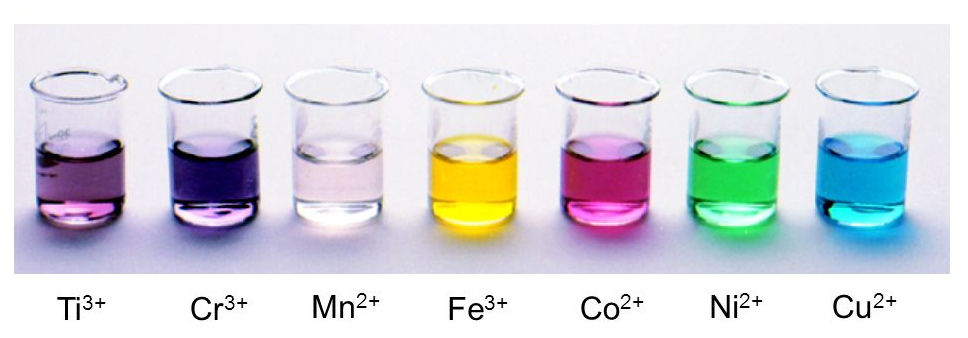
\includegraphics[width=12cm]{immagini/ioni_complessi.png}
\end{figure}

Inoltre questi complessi danno luogo a soluzioni colorate, sebbene i sali anidri (cioè senza acqua) non presentano tali colorazioni. Il colore è dovuto allora al complesso che si forma. La reazione del catione metallico e un certo numero di molecole di acqua è una reazione acido-base: l'acqua è il doppietto ed è la base di Lewis, lo ione metallico ha orbitali vuoti e quindi può accettare coppie di elettroni, pertanto è l'acido di Lewis.

\vspace{0.2cm}Esempi:
$$\ce{Be^{2+}(aq) + 4H_2O(l) <--> [Be(H_2O)_4]^{2+}(aq)}$$

Questo ione viene coordinato da 4 molecole d'acqua, formando un complesso tetraedrico, ossia gli ossigeni dell'H$_2$O sono disposti ai vertici di un tetraedro.

Quindi in acqua non c'è un mescolamento casuale, si formano delle geometrie ben precise nei complessi. Le molecole di acqua costituiscono l'\textit{intorno di coordinazione}.

Anche in questo esempio lo ione berillio è un acido di Lewis e l'acqua è la base di Lewis.

\subsection{Lo ione idronio H$_3$O$^+$}
Abbiamo detto che etichettiamo acidi i composti che cedono un protone. Possiamo allora immaginare che l'idrogeno diventi H$^+$ più un elettrone e$^-$.

Il protone H$^+$ ha dimensioni di 0.0015 pm, mentre gli atomi hanno dimensioni tra i 50 e i 200 pm, ciononostante la sua carica è comunque +1 come quella di uno ione. Ne segue che il rapporto tra carica e raggio per l'H$^+$ è molto più grande di quello degli ioni. A causa di ciò, il protone non può esistere da solo in un liquido o in un solido: si associa a qualunque cosa pur di diminuire il rapporto carica raggio.

In acqua si associa ad una molecola d'acqua per formare lo ione idronio $\rm H_3O^+$. Così facendo la carica resta +1 ma le dimensioni della molecola crescono.

$$\ce{H^+(g) + H_2O(g) <--> H_3O^+(gas)}$$

Quando questa reazione avviene, vista l'elevata tendenza del protone ad associarsi con altre specie chimiche per ridurre il rapporto carica raggio, si liberano 720 kJ/mol.

Va da ricordare che quando l'idrogeno perde un protone ha un potenziale di ionizzazione di 1311 kJ/mol (\ce{H <--> H^+ + e^-}).

\vspace{0.2cm}Consideriamo adesso la stessa reazione in acqua liquida:

$$\ce{H^+(g) + H_2O(l) <--> H_3O^+(aq)}$$

In questo caso lo ione H$^+$ gassoso viene catturato da dell'acqua liquida per formare lo ione $\rm H_3O^+$ in acqua, quindi il protone gassoso si idrata perché si somma ad una molecola d'acqua in soluzione acquosa.

Il $\Delta$H stavolta è di 1090 kJ/mol, cioè l'acqua permette una grande stabilizzazione al protone.

\vspace{0.2cm}Quindi quando discutiamo di speci acide in acqua stiamo discutendo della presenza di ioni $\rm H_3O^+$, in quanto qualunque acido A che reagisce con l'acqua darà luogo alla formazione della specie A$^-$ (circondata anch'essa da molecole d'acqua coordinate) e dello ione $\rm H_3O^+$:
$$\ce{HA + H_2O <--> H_3O^+ + A^-}$$

Mettiamo una doppia freccia perché queste reazioni la maggior parte delle volte sono equilibri (metterla sempre può avere significato matematico ma non chimico!).
\subsection{Acidi e basi}

\vspace{0.2cm}\ce{HNO_3(aq) + H_2O(l) -> H_3O^+(aq) + NO_3^-(aq)}

\vspace{0.2cm}L'acido nitrico in acqua si dissocia, liberando un protone che si somma all'acqua che diventa ione $\rm H_3O^+$. Resta lo ione $\rm NO_3^-$.

Etichettiamo come acido la specie $\rm HNO_3$ e come base coniugata la specie $\rm NO_3^-$. Chiaramente però se $\rm HNO_3$ è l'acido vuol dire che in soluzione c'era una base, che è l'$\rm H_2O$. Quindi in questa reazione l'acqua si comporta da base e $\rm H_3O^+$ è il suo acido coniugato.

Abbiamo quindi coppie coniugate, in modo da avere un acido e una base sia a sinistra che a destra. Diciamo coniugate perché le otteniamo a partire dagli acidi e dalle basi iniziali.

\vspace{0.2cm}\ce{NH_4^+(aq) + H_2O(l) <--> H_3O^+(aq) + NH_3(aq)}

\vspace{0.2cm}Lo ione ammonio $\rm NH_4^+$ libera un protone e diventa ammoniaca $\rm NH_3$, quindi lo ione ammonio è la specie acida e l'ammoniaca la sua base coniugata. Se lo ione ammonio libera un protone, è indispensabile che ci sia una specie che la acquisti. Tale specie è l'acqua, che pertanto risulta essere una base perché acquista il protone liberato. Essa inoltre genera la specie $\rm H_3O^+$ che è il suo acido coniugato.

Anche in questa reazione abbiamo sia a sinistra che a destra una coppia acido-base.

\vspace{0.2cm}\ce{HSO_4^-(aq) + H_2O(l) <--> H_3O^+(aq) + SO_4^{2-}(aq)}

\vspace{0.2cm}Il solfato acido può cedere un protone e diventare $\rm SO_4^-$, quindi esso è la base coniugata dell'$\rm HSO_4^-$. Lo ione $\rm H_3O^+$ sarà invece l'acido della base $\rm H_2O$ che acquista il protone ceduto. Anche qui ci sono due coppie acido-base.

\vspace{0.2cm}In queste prime tre reazioni l'acqua è sempre la base.

\vspace{0.2cm}\ce{NH_3(aq) + H_2O(l) <--> NH_4^+(aq) + OH^-}

\vspace{0.2cm}Stavolta l'ammoniaca strappa un protone all'acqua, formando lo ione ammonio. Dell'acqua, tolto un protone, resta la specie OH$^-$. Quindi, contrariamente a sopra, l'acqua sarà l'acido e l'ammoniaca la base. Avremo poi che lo ione ammonio è l'acido e lo ione OH$^-$ è la base. Quindi OH$^-$ è la base coniugata dell'acido $\rm H_2O$, $\rm NH_4^+$ l'acido coniugato della base $\rm NH_3$.

\vspace{0.2cm}\ce{CO_3^{2-}(aq) + H_2O(l) <--> HCO_3^-(aq) + OH^-(aq)}

\vspace{0.2cm}Lo ione carbonato è una base, perché in questa reazione strappa un protone all'acqua (ne può strappare più di uno) diventando ione $\rm HCO_3^-$, che quindi sarà il suo acido coniugato. L'acqua, che ha ceduto un protone, è un acido, e la sua base coniugata è OH$^-$. Abbiamo ancora due coppie acido-base.

\vspace{0.2cm}$\bullet$\textbf{Acidi poliprotici}
\begin{center}
\begin{tabular}{lllll}
    $\rm H_2SO_4$ & $\rm H_3PO_4$ & $\rm H_2CO_3$ & $\rm H_2S$ & $\rm H_2C_2O_4$\\
    acido solforico & acido fosforico & acido carbonico & acido solfidrico & acido ossalico    
\end{tabular}
\end{center}
\vspace{0.2cm}$\bullet$\textbf{Basi poliprotiche}
\begin{center}
\begin{tabular}{lllll}
    $\rm SO_4^{2-}$ & $\rm PO_4^{3-}$ & $\rm CO_3^{2-}$ & $\rm S^{2-}$ & $\rm C_2O_4^{2-}$\\
    ione solfato & ione fosfato & ione carbonato & ione solfuro & ione ossalato    
\end{tabular}
\end{center}

Degli acidi poliprotici abbiamo le basi corrispondenti. Per ottenere queste non è necessario partire dagli acidi, possiamo partire da loro sali (anche perché queste dissociazioni non avverrebbero mai così totalmente, si tratta in larga misura di acidi deboli): solfuri, carbonati, fosfati ecc, che sono elettroliti forti e pertanto totalmente dissociati, per dissociazione ci danno gli ioni $\rm S^{2-}$, $\rm CO_3^{2-}$, $\rm PO_4^{3-}$ ecc.

Tali speci strapperanno protoni all'acqua, comportandosi da base. Ne segue che l'acqua si comporterà da acido, perché cederà protoni.

\vspace{0.2cm}Consideriamo ad esempio il fosfato di sodio $\rm Na_3PO_4$. Esso si dissocia totalmente in ioni sodio Na$^+$ e ioni fosfato $\rm PO_4^{3-}$. Quest'ultimo strapperà protoni all'acqua, diventando $\rm HPO_4^{2-}$, $\rm H_2PO_4^-$ e $\rm H_3PO_4$. L'acqua allora sarà un acido e lo ione fosfato una base.

Questi ioni sono basi fortissime, ma non lo avremmo potuto dire con la teoria di Arrhenius.
\subsection{Anfoliti}

\ce{HCl(aq) + H_2O(l) -> H_3O^+(aq) + Cl^-(aq)}

\vspace{0.2cm}In questa reazione l'acqua acquista un protone, quindi è una base.

\vspace{0.2cm}\ce{NH_3(aq) + H_2O(l) <--> NH_4^+(aq) + OH^-(aq)}

\vspace{0.2cm}Qui l'acqua cede un protone, quindi è un acido.

\vspace{0.2cm}\ce{HCO_3^-(aq) + H_2O(l) <--> H_3O^+(aq) + CO_3^{2-}}

\vspace{0.2cm}\ce{HCO_3^-(aq) + H_2O(l) <--> H_2CO_3(aq) + OH^-}

\vspace{0.2cm}Con lo ione bicarbonato in acqua possono avvenire due reazioni: in una esso cede un protone all'acqua, che quindi sarebbe una base perché lo acquista, diventando ione carbonato, nell'altra invece strappa un protone, diventando acido carbonico, e l'acqua che cederebbe il protone si comporterebbe da acido.

\vspace{0.2cm}In questi esempi l'acqua a volte si comporta come acido, altre come base. I composti che hanno questa proprietà si chiamano \textbf{composti anfoteri} o \textbf{anfoliti}. Essi sono composti per cui il comportamento di acido o di base dipende fortemente dall'ambiente in cui si trovano. Hanno quindi un comportamento intermedio.

Ne è un esempio l'acqua, che prende parte attivamente alla reazione comportandosi da acido o da base.

\vspace{0.2cm}Ricorda: ciò che sfuggiva ad Arrhenius era il ruolo dell'acqua!

\vspace{0.2cm}Un altro esempio di anfolita è l'idrossido di alluminio Al(OH)$_3$:

\begin{figure}[htp]
    \centering
    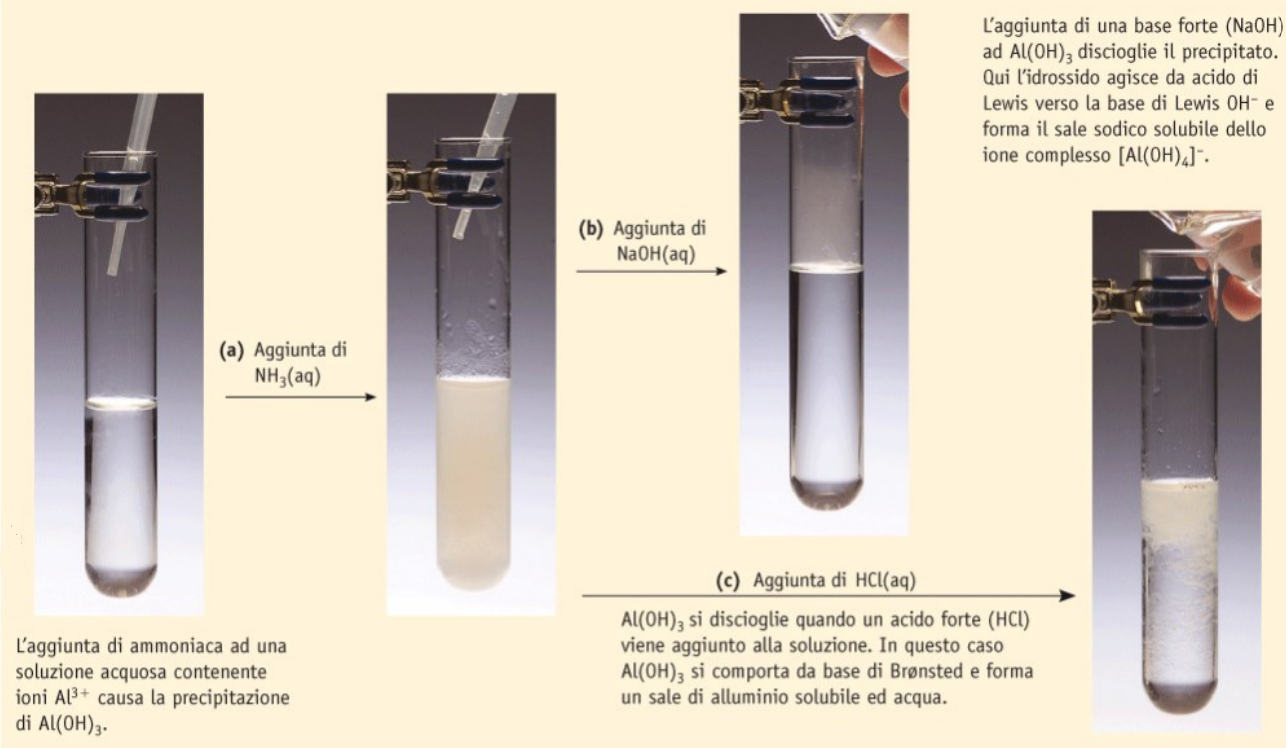
\includegraphics[width=12cm]{immagini/anfoliti.png}
\end{figure}

Immaginiamo di avere un sale di alluminio solubile in acqua. Se fosse in soluzione non ce ne accorgeremmo, in quanto la soluzione sarebbe limpida e incolore. Se aggiungiamo ammoniaca, che è una base, si forma un precipitato gelatinoso bianco, che è l'idrossido di alluminio.

L'$\rm Al(OH)_3$ si è formato dopo aver aggiunto l'ammoniaca che è una base debole, ossia non si dissocia totalmente.

Immaginiamo di aggiungere un'ulteriore base, questa però più forte. Essa sarà l'idrossido di sodio NaOH. Ci si accorge che il precipitato ottenuto prima si risolubilizza, si riscioglie, e la soluzione sarà di nuovo limpida e incolore. Ciò succede perché avevamo la specie neutra $\rm Al(OH)_3$ e ora si è formata la specie $\rm [Al(OH)_4]^-$, cioè un anione. Tale complesso si forma grazie all'$\rm OH^-$ proveniente dall'NaOH, quindi adesso in soluzione abbiamo lo ione $\rm Na^+$ e lo ione $\rm [Al(OH)_4]^-$. Abbiamo cioè formato un sale complesso di sodio detto \textit{alluminato di sodio}, perché abbiamo formato un complesso con lo ione alluminio al centro di un tetraedro i cui quattro vertici sono occupati dagli ossigeni dei gruppi $\rm OH^-$, il quale ha carica totale -1.

Quindi con l'ammoniaca abbiamo ottenuto un precipitato, con l'NaOH lo abbiamo sciolto.

Se infine aggiungiamo un acido forte, ad esempio HCl, succede che si forma di nuovo il precipitato, ossia l'idrossido di alluminio ottenuto si scioglie in NaOH e riprecipita in acido cloridrico. Questo comportamento ci indica che l'idrossido di alluminio è un composto anfotero. Infatti esso si scioglie in una base forte, cioè si comporta da acido di Lewis, e di fatto accetta un doppietto di elettroni, mentre la specie $\rm OH^-$ proveniente da NaOH è la base di Lewis che dona elettroni. In questo modo si forma il sale $\rm Na[Al(OH)_4]$.

Se invece aggiungiamo un acido forte l'idrossido di alluminio diventa una base di Brönsted, perché forma un sale di alluminio che si scioglie in acqua.

Abbiamo quindi una specie che, a seconda che si usi un acido o una base, assume il comportamento necessario per il partner, cioè a volte si comporta da acido di Lewis, altre da base di Brönsted.

\vspace{0.2cm}Vediamo di spiegare in altri termini.

Se in acqua abbiamo un sale del tipo AlX, esso sarà dissociato in ioni $\rm Al^{3+}$ e $\rm X^{3-}$.

Quando aggiungiamo ammoniaca in acqua avviene la reazione

$$\ce{NH_3 + H_2O <--> NH_4^+ OH^-}$$

Questi ioni $\rm OH^-$ che si formano vanno a legarsi con gli ioni $\rm Al^{3+}$, formando l'idrossido di alluminio $\rm Al(OH)_3$.

La reazione che effettivamente avviene è

$$\ce{Al^{3+}(aq) + 3NH_3(aq) + 3H_2O(l) <--> AlOH_3(s) + 3NH_4^+(aq)}$$

A questo punto ci sono due possibilità: o aggiungiamo una base forte o aggiungiamo un acido forte.

\vspace{0.2cm}1) Aggiungiamo una base forte, ad esempio idrossido di sodio NaOH. La reazione che avviene sarà

$$\ce{Al(OH)_3(aq) + NaOH <--> [Al(OH)_4]^- + Na^+}$$

In essa l'$\rm Al(OH)_3$ ha assorbito una coppia di elettroni (se ci pensiamo, sull'$\rm OH^-$ c'è un doppietto), quindi si è comportato da acido di Lewis

\vspace{0.2cm}2)Aggiungiamo invece un acido forte, ad esempio acido cloridrico

$$\ce{Al(OH)_3(aq) + 3HCl -> AlCl_3 + 3H_2O}$$

Siccome l'HCl cede protoni, ci deve essere qualcuno che li accetta,ossia l'$\rm Al(OH)_3$. Ma se assorbe protoni allora è una base di Brönsted.

\vspace{0.2cm}\textbf{Altri esempi}

\vspace{-0.3cm}\begin{center}
    \footnotesize\begin{tabular}{|p{5.2cm}p{5.4cm}p{3.8cm}|}
    \hline
    \textbf{Forma acida} & \textbf{Forma anfiprotica} & \textbf{Forma basica}\\
    \hline
    &&\\[-1.2ex]
    $\rm H_2S$ (acido solfidrico o solfuro & $\rm HS^-$ (ione idrogeno solfuro) & $\rm S^{2-}$ (ione solfuro)\\
    di idrogeno)&&\\[0.7ex]
    $\rm H_3PO_4$ (acido fosforico) &  \hspace{-0.2cm}$\left[
\begin{aligned}
    \text{H}_2\text{PO}_4^- \; \text{(ione diidrogeno fosfato)}\\
    \text{HPO}_4^{2-} \text{(ione idrogeno fosfato)} \hspace{0.4cm}
\end{aligned}
\right .$
 & $\rm PO_4^{3-}$ (ione fosfato)\\[3ex]
 $\rm H_2CO_3$ (acido carbonico) & $\rm HCO_3^-$ (ione idrogeno carbonato& $\rm CO_3^{2-}$ (ione carbonato)\\
 & o ione bicarbonato) &\\[0.7ex]
 $\rm H_2C_2O_4$ (acido ossalico) & $\rm HC_2O_4^-$ (ione idrogeno ossalato) & $\rm C_2O_4^{2-}$ (ione ossalato)\\[0.7ex]
 \hline
    \end{tabular}
\end{center}

Concentriamoci sulle forme basiche:

\begin{itemize}
    \item Lo ione solfuro $\rm S^{2-}$ è una base. Infatti se mettessimo un suo sale in acqua come ad esempio solfuro di sodio $\rm Na_2S$, questo si dissocerebbe in $\rm 2Na^+$ e $\rm S^{2-}$. Quest'ultimo ione strapperebbe protoni all'acqua per formare la specie $\rm HS^-$ e lasciando lo ione $\rm OH^-$. Nei fatti quindi tale specie si sta comportando da base;
    \item Lo ione fosfato $\rm PO_4^{3-}$ può strappare uno o più protoni all'acqua. Ogni volta che ne strappa uno resta uno ione $\rm OH^-$ in eccesso. Si comporta quindi da base;
    \item Ione carbonato $\rm CO_3^{2-}$: analogo al solfuro;
    \item Ione ossalato $\rm C_2O_4^{2-}$: analogo al solfuro.
\end{itemize}

Questi ioni non possono rientrare nella definizione di Arrhenius secondo cui una base è una specie in grado di cedere ioni $\rm OH^-$ in soluzione, in quanto essi non sono presenti nelle speci appena viste.

Ne segue che etichettare basica una specie non significa che necessariamente gli ioni $\rm OH^-$ debbano essere presenti in quella specie. Ne sono un esempio questi ioni, che diventano basi se sciolti in acqua. Viceversa, se mettiamo i sali (apparentemente neutri) in soluzione, questa diventa basica.